%%%%%%%%%%%%%%%%%%%%%%%%%%%%%%%%%%%%%%%%%%%%%%%%%%%%%%%%%%%%%%%%%
% Dissertacao de Mestrado / Dept Fisica, CFM, UFSC              %
% Andre@UFSC - 2011                                             %
%%%%%%%%%%%%%%%%%%%%%%%%%%%%%%%%%%%%%%%%%%%%%%%%%%%%%%%%%%%%%%%%%

%:::::::::::::::::::::::::::::::::::::::::::::::::::::::::::::::%
%                                                               %
%                          Capítulo 5                           %
%                                                               %
%:::::::::::::::::::::::::::::::::::::::::::::::::::::::::::::::%

%***************************************************************%
%                                                               %
%                           Conclusao                           %
%                                                               %
%***************************************************************%

\chapter{Conclusões e perspectivas}
\label{sec:conclusao}


%***************************************************************%
%                                                               %
%                    Conclusao - este trabalho                  %
%                                                               %
%***************************************************************%

\section{Este trabalho}

Este estudo teve como objetivo principal explorar o uso de bancos de dados em
astronomia. Com a previsão de um dilúvio de dados, é de extrema importância que
sejam desenvolvidas técnicas e ferramentas adequadas para absorver este volume
de dados.

A importação do catálogo do \starlight para um banco de dados relacional foi uma
tarefa relativamente simples. O uso de um banco de dados relacional, neste caso
{\em MS SQL Server}, facilitou muito o gerenciamento do catálogo. As diversas
ferramentas disponíveis permitem que se manipule os dados de uma forma
eficiente. Em especial, grande parte do presente trabalho foi feito nos
ambientes {\em CasJobs}, tanto do \starlight quanto do \SDSS e do \galex. O
catálogo tem sido usado intensamente por colaboradores do \starlight em São
Paulo e na Espanha, além de ter diversos usuários espalhados pelo mundo (Figura
\ref{fig:AcessosStarlight}).

\begin{figure}
	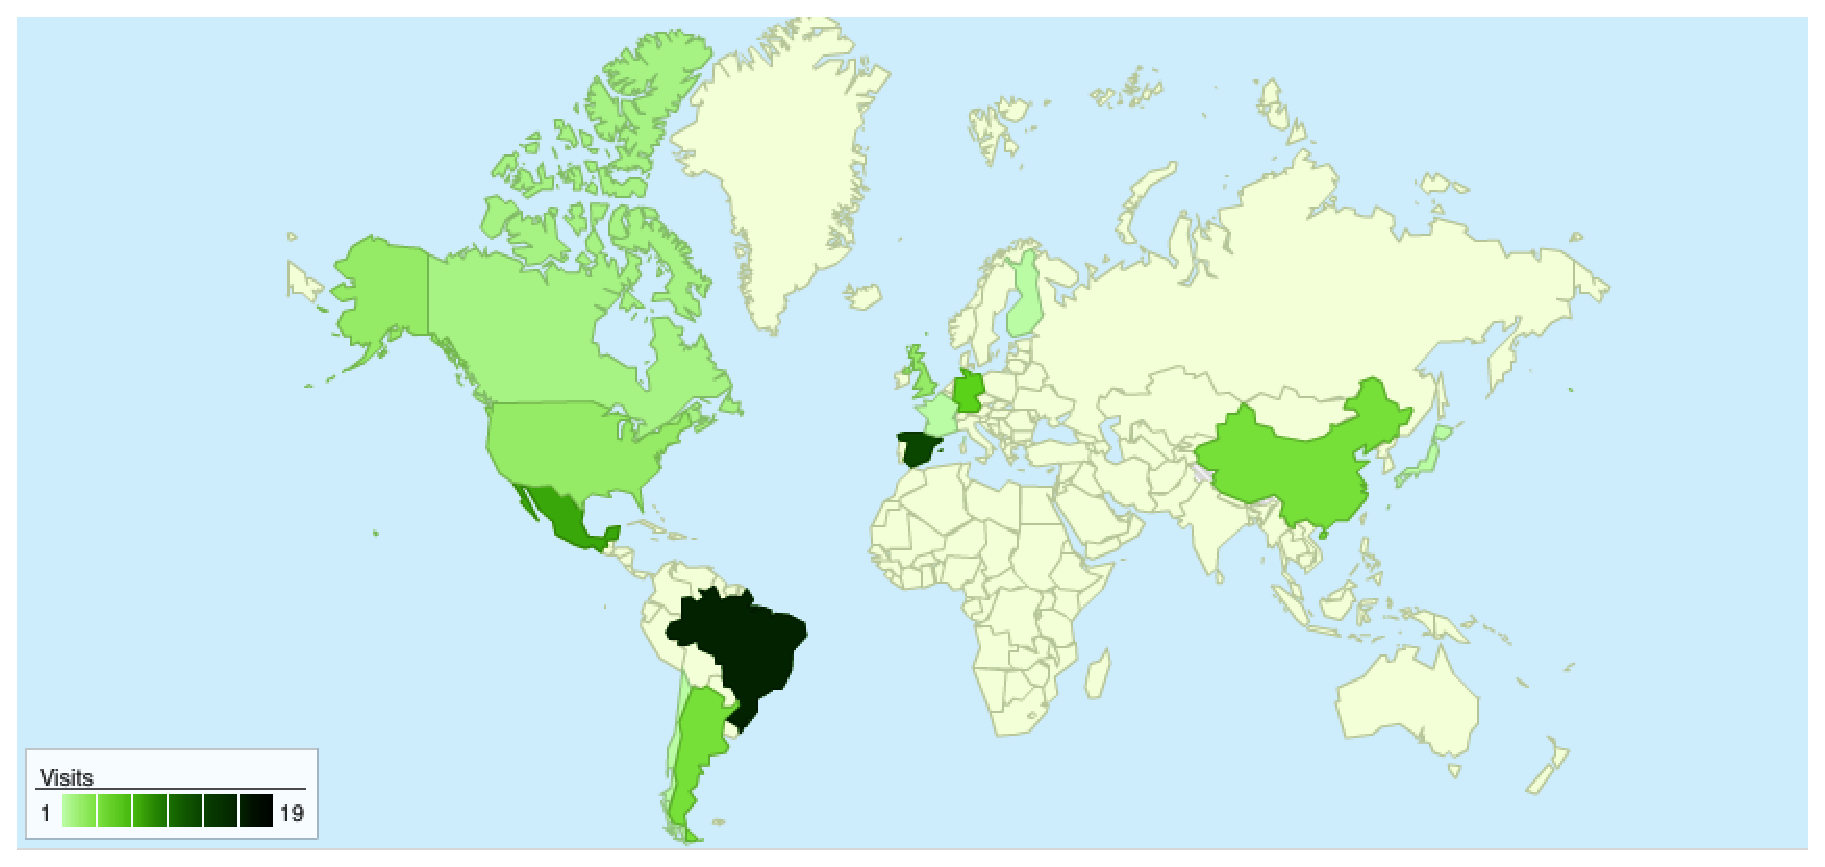
\includegraphics[width=\textwidth]{figuras/starlight-analytics.eps}
	\caption[Localização dos acessos ao {\em CasJobs} do \starlight.]
	{Localização dos acessos ao {\em CasJobs} do \starlight. O número de acessos é
	referente ao mês de novembro de 2011.}	
	\label{fig:AcessosStarlight}
\end{figure}

Por si só, o uso dos dados provenientes de um único {\em survey} de grande porte
tem o potencial de gerar resultados até então inimagináveis. A identificação
cruzada de objetos em {\em surveys} diferentes, por sua vez, promete ampliar e
muito este espaço de possibilidades. O esforço de \citet{Budavari2009},
utilizando as técnicas de indexação espacial descritas por \citet{Kunszt2001},
na identificação cruzada de objetos entre \SDSS e \galex é de suma importância
neste sentido: a maioria dos {\em surveys} atuais provê (ou planeja) formas de
integração com o \SDSS e outros {\em surveys}. Esta informação cruzada foi
utilizada para obter os dados fotométricos em UV dos objetos do catálogo do
\starlight. Assim, o banco de dados agora contém as propriedades físicas de
quase um milhão de galáxias, os seus correspondentes parâmetros observacionais
provenientes do \SDSS, e as magnitudes UV absolutas e corrigidas (poeira e
correção $k(z)$) para aproximadamente $170$ mil galáxias, obtidas pelo \galex.

Como um estudo de caso, foi montada uma amostra de galáxias do catálogo do
\starlight, com as suas propriedades físicas, algumas linhas de emissão e
fotometria óptica e UV (chamada amostra \starlightUV). Dados os critérios de
seleção da amostra, a extração da amostra resume-se a executar uma {\em query}
no {\em CasJobs} e obter o seu resultado em um arquivo no formato desejado, FITS
por exemplo. É claro, este processo pode ser repetido caso os critérios de
seleção mudem (o que foi feito muitas vezes neste estudo, diga-se de passagem).
Ainda assim, a ideia é abandonar a cultura de ter todo o conjunto de dados do
catálogo presentes no computador do usuário. Com os catálogos imensos que estão
sendo planejados (J-PAS e LSST, por exemplo), é bastante provável que este seja
o caminho mais eficiente a se seguir.

No capítulo \ref{sec:Analise} mostrou-se que as classes de galáxias da amostra
\starlightUV, segundo os critérios de classificação descritos por
\citet{CidFernandes2011}, tendem a ocupar regiões distintas do diagrama
cor--cor. Pôde-se notar, nos diagramas cor--cor para as propriedades físicas das
galáxias, que a distribuição de RG tem um espalhamento considerável na direção
das AGN e SF. Com um exercício simples, foi possível verificar que este
espalhamento é devido não somente à incerteza nas medidas, mas também por se
utilizar uma classificação discreta sobre fenômenos que são de natureza
contínua.

Tecnicamente, as PG e as RG deveriam ser essencialmente as mesmas, com as RG
apresentando linhas de emissão fracas. Em geral as propriedades físicas destas
duas classes apresentam uma sobreposição considerável, como pode ser visto nos
diagramas cor--cor (Figuras \ref{fig:ATFluxColor} até \ref{fig:AVColor}), e são
distintas das duas classes AGN. Ainda assim, é preciso ter em mente de que
parece haver diferenças sistemáticas entre as PG e as RG. É preciso estudar
estas diferenças mais a fundo.


%***************************************************************%
%                                                               %
%                  Conclusao - trabalhos futuros                %
%                                                               %
%***************************************************************%

\section{Trabalhos futuros}

O estudo da amostra \starlightUV presente neste trabalho foi feito de forma
superficial. A intenção foi apenas demonstrar uma forma de trabalhar com dados
provenientes de diversos catálogos. As observações feitas no capítulo
\ref{sec:Analise} são em geral de caráter qualitativo. Entretanto, os dados
sugerem que existe uma contaminação entre as classes de galáxias. Um provável
candidato é o erro na medida de \WHa na amostra. Isto causa uma contaminação de
galáxias SF e wAGN nas RG. É preciso determinar se o erro nas medidas é,
sozinho, capaz de explicar esta contaminação, ou se ela é inerente à
classificação simplificada adotada.

A síntese feita pelo \starlight levou em conta apenas a região óptica do
espectro, mas os modelos de SSP utilizados possuem dados que se estendem até
além do UV. É possível calcular a magnitude UV esperada para uma galáxia dados
os seus componentes determinados na síntese. Porém, para poder comparar os dados
previstos pela síntese com os observados, é preciso garantir que os dados são
compatíveis. A fotometria do \galex é integrada sobre toda a galáxia. Já os
espectros do \SDSS, foram obtidos utilizando uma fibra com aproximadamente $3$
segundos de arco. Cada fibra não captura, necessariamente, toda a luz das uma
galáxia. Em geral a fração da luz de uma galáxia capturada pela fibra varia com
o tamanho da galáxia e o seu {\em redshift}. Assim, por exemplo, regiões de
formação estelar, com emissão em UV significativa, que estão na periferia de uma
galáxia podem ter sido excluídas. Para fazer uma comparação adequada é
necessário refazer a fotometria dos objetos \galex utilizando uma abertura
equivalente ao tamanho da fibra usada no \SDSS. Esta comparação pode ajudar a
determinar a acurácia dos modelos de SSP em UV, além de testar a lei de
atenuação usada na síntese\footnote{As leis de atenuação
\citet*[CCM]{Cardelli1989} e \citet*{Calzetti1994} têm previsões diferentes em
UV devido à presença ou não da corcova em $2175\,\text{\AA}$.}. Outra
possibilidade é usar esta fotometria UV limitada ao diâmetro da fibra como
pontos extras do espectro de entrada do \starlight. Desta forma espera-se que o
ajuste possa ser mais sensível à formação estelar recente, e possa separar uma
formação estelar fraca de objetos velhos e quentes, como anãs brancas, por
exemplo. A versão mais recente do \starlight já está preparada para trabalhar
com dados fotométricos em conjunto com espectrais.

Embora a seleção da amostra tenha sido feita no banco de dados, uma boa parte da
análise foi feita num computador pessoal. Isto custou diversas iterações de
extração e diagnóstico da amostra. Alguns procedimentos como a classificação das
galáxias e histogramas de propriedades físicas poderia ser feita diretamente no
servidor. O próximo passo, com relação ao banco de dados do \starlight, é criar
ferramentas de diagnóstico que rodem no servidor. A ideia é que estas
ferramentas possam ser facilmente estendidas e abstraiam a forma como as
informações estão armazenadas no banco de dados.

Esta forma de trabalho deve se tornar a regra nos próximos anos. Pode-se pensar
que será possível armazenar dezenas de petabytes obtidas pelo LSST no computador
do pesquisador, dado o crescimento que vem ocorrendo na densidade de
armazenamento. Entretanto, é preciso cautela. \citet{Way2011} compara o
crescimento da densidade de armazenamento com a largura de banda de
entrada/saída (E/S) e a velocidade de processamento. Embora uma {\em query} em
geral escale linearmente com o tamanho de um banco de dados, as operações
científicas comumente aplicadas aos dados incluem classificação, cálculo de
distância e densidade, por exemplo, e são geralmente de complexidade $O(N^2)$.
Ou seja, mesmo que seja possível armazenar todo o conteúdo de um {\em survey}
deste porte, é bastante provável que uma abordagem tradicional, acessando os
dados de forma sequencial, esbarre na limitação de E/S e poder computacional.
Tudo indica que a aposta mais segura seja manter os dados em centros de
processamento de dados ({\em data centers}) poderosos, possivelmente espalhados
geograficamente para melhorar a velocidade do acesso.

% End of this chapter
